\documentclass[12pt, a4paper]{article}
\usepackage[utf8]{inputenc}
\usepackage[T2A]{fontenc}
\usepackage{indentfirst, setspace}
\usepackage{tabularx, multirow}
\usepackage[normalem]{ulem}
\usepackage[style=russian]{csquotes}
\usepackage[english,russian]{babel}
\usepackage{hyperref}
\usepackage{ragged2e}
\usepackage{caption}
\usepackage{wrapfig}
\usepackage{amsmath}
\usepackage{tikz}
\makeatletter
\def\@biblabel#1{#1. }
\makeatother
\captionsetup{labelsep=endash}
\usepackage{listings}
\linespread{1.3}
\lstset{
  language=C++,
  basicstyle=\ttfamily\small,
  keywordstyle=\color{blue},
  breaklines=true,
  commentstyle=\color{green},
  stringstyle=\color{red},
  extendedchars=\true,
  showstringspaces=false,
  keepspaces=true,
}

\usepackage[left=2cm,right=2cm,
    top=2cm,bottom=2cm,bindingoffset=0cm]{geometry}\begin{document}
\begin{titlepage}
     \fontsize{12}{12}\selectfont

  {\centering

   \begin{bf}

    \begin{wrapfigure}{l}{10mm}
        
\includegraphics[width=17mm]{photo_2023-12-07_04.12.41.jpeg}
    \end{wrapfigure}


    \noindent Министерство науки и высшего образования Российской Федерации

    \noindent Федеральное государственное бюджетное образовательное учреждение высшего образования

    \noindent \enquote{Московский государственный технический университет

     \noindent имени Н.Э. Баумана

     \noindent (национальный исследовательский университет)}

    \noindent (МГТУ им. Н.Э. Баумана)

   \end{bf}
  }

  \vspace{0.4cm}

  {\setstretch{0.1}
   \noindent\rule{\textwidth}{1mm}
   \noindent\rule{\textwidth}{0.5mm}

  }

  \fontsize{14}{21}\selectfont

  \noindent\begin{tabularx}{\textwidth}{l >{\centering\arraybackslash}X}
   ФАКУЛЬТЕТ & \flqq Фундаментальные Науки\frqq \\ \cline{2-2}

   КАФЕДРА & ФН-12 \flqq Математическое моделирование\frqq \\ \cline{2-2}
  \end{tabularx}

  \vspace{1cm}


  \begin{center}
   \begin{bf}

    \fontsize{24}{36}\selectfont
    ОТЧЕТ

    \fontsize{20}{30}\selectfont
    ПО РК 1:

    Метод перебора
   \end{bf}
  \end{center}

  \fontsize{14}{21}\selectfont
  \vspace{5cm}


  \noindent\begin{tabularx}{\textwidth}{ X >{\centering}p{4cm} p{1cm} c }
   Студент: & & & Мациевский И. М. \\ \cline{2-2} \cline{4-4}
   & \fontsize{10}{15}\selectfont дата, подпись & & \fontsize{10}{15}\selectfont Ф.И.О. \\
   Преподаватель: & & & Волкова Л. Л.\\ \cline{2-2} \cline{4-4}
   & \fontsize{10}{15}\selectfont дата, подпись & & \fontsize{10}{15}\selectfont Ф.И.О.
   \end{tabularx}

  \vspace{\fill}

  \begin{center}
   \it{Москва}, 2023
  \end{center}

  \thispagestyle{empty}
\end{titlepage}\newpage
\tableofcontents
\newpage
\section*{Введение}
\addcontentsline{toc}{section}{Введение}
\justifying
\textbf{Цель:}
Решить подзадачу задачи коммивояжера, получить навык 
реализации алгоритмов.
Реализовать метод полного перебора в графе: дан граф на $N$ 
вершин, требуется перебрать все возможные решения 
задачи коммивояжера --- кортежи $N$ городов.
\section{Аналитическая часть}
\subsection{Задача коммивояжера}
\textbf{Задача коммивояжера ---} это классическая задача 
комбинаторной оптимизации, которая формулируется следующим 
образом: 
имеется граф, в котором вершины представляют города, а рёбра — 
пути между городами. Каждому ребру сопоставлен вес, который обычно 
представляет собой расстояние или стоимость перемещения между 
соответствующими городами. Задача состоит в том, чтобы найти самый 
выгодный (кратчайший или наименее затратный) маршрут, проходящий 
через каждый город ровно один раз и возвращающийся в исходный 
город.
\subsection{Метод полного перебора}
\textbf{Метод полного перебора ---} это способ решения задачи 
коммивояжера, при котором алгоритм перебирает все возможные 
варианты посещения вершин графа и выбирает оптимальный. Для задачи 
коммивояжера метод полного перебора проверяет все возможные 
порядки 
посещения городов и находит тот, который является минимальным по 
суммарному пройденному расстоянию.
Преимуществом этого метода является простота его написания, но он
неэффективен из-за проверки всех возможных маршрутов.
\section{Конструкторская часть}
\begin{enumerate}
	\item Создать два вектора: $free$ и $ans$ --- в первом 
	хранятся свободные вершины, то есть те, которые пока не 
	включены в данный маршрут, а во втором те, которые уже входят 
	в него, изначально вектор $free$ пуст, а в векторе $ans$ 
	хранятся вершины в любой последовательности. Инициализируется 
	переменная $last$, изначально $last = 
	ans[N-1]$. $ans$ добавляется в файл всех перестановок
	\item Далее следует найти вершину с минимальным номером, 
	который при этом больше, чем $last$. 
	\item Если такая вершина нашлась, она добавляется в вектор 
	$ans$, после чего в него в порядке возрастания записываются 
	оставшиеся вершины, вектор $free$ отчищается, вектор $ans$ 
	записывается в файл со всеми маршрутами.
	\item Если такой вершины нет и при этом вектор $ans$ пуст, все 
	маршруты найдены, программа завершается. Если же вектор $ans$ 
	не пуст, то последний элемент переносится из вектора $ans$ в 
	вектор $free$, при этом переменная $last$ принимает его 
	значение.
\end{enumerate}
\section{Технологическая часть}
Для реализации выбран язык C++.
Функции, реализованные в проекте:
\begin{enumerate}
	\item $show\_one\_dim$ --- выводит на экран одномерный вектор;
	\item $write\_to\_f$ --- записывает вектор в файл.
\end{enumerate}
\newpage
Для реализации выбран язык C++.
На листинге 1 представлена реализация программы
(Реализация~\ref{lst:label1}).
\begin{lstlisting}[caption={Исходный код}, label={lst:label1}]
#include <iostream>
using namespace std;
#include <vector>
#include <fstream>

void show_one_dim(const vector<int>& vec) {
  for (int i = 0; i < vec.size(); i++) {
    cout << vec[i] + 1 << " ";
  }
}

void write_to_f (vector<int>&vec, fstream &file) {
    for (int i = 0; i < vec.size(); i++) {
      file << vec[i] + 1 << " ";
    }
    file << endl;
}


int main() {
    fstream file("/Users/ilya/Downloads/Типы и структуры данных 2 курс, 1 семестр/complet_search/permutations.txt");
    int n;
    cin >> n;
    vector<int> free;
    vector<int> ans;
    for (int i = 0; i < n; i++) {
        ans.push_back(i);
    }
    int last;
    last = ans[n - 1];
    write_to_f(ans, file);
    ans.pop_back();
    free.push_back(last);
    while (1) {
        int new_el = n + 1;
        for (int i = 0; i < free.size(); i++) {
            if (free[i] > last) {
                new_el = min(free[i], new_el);
            }
        }
        if (new_el == n + 1) {
            if (ans.empty()){
                //show_one_dim(free);
                write_to_f(ans, file);
                break;
            }
            last = ans[ans.size() - 1];
            ans.pop_back();
            free.push_back(last);
        }
        else {
            ans.push_back(new_el);
            erase(free, new_el);
            sort(free.begin(), free.end());
            for (int i = 0; i < free.size(); i++) {
                ans.push_back(free[i]);
            }
            free.clear();
            write_to_f(ans, file);
        }
    }
    file.close();
    return 0;
}
\end{lstlisting}

\textbf{Примеры работы.}
\begin{enumerate}
	\item $N=1$, то есть дерево из 1 вершины.
	\begin{figure}[h]
  		\center{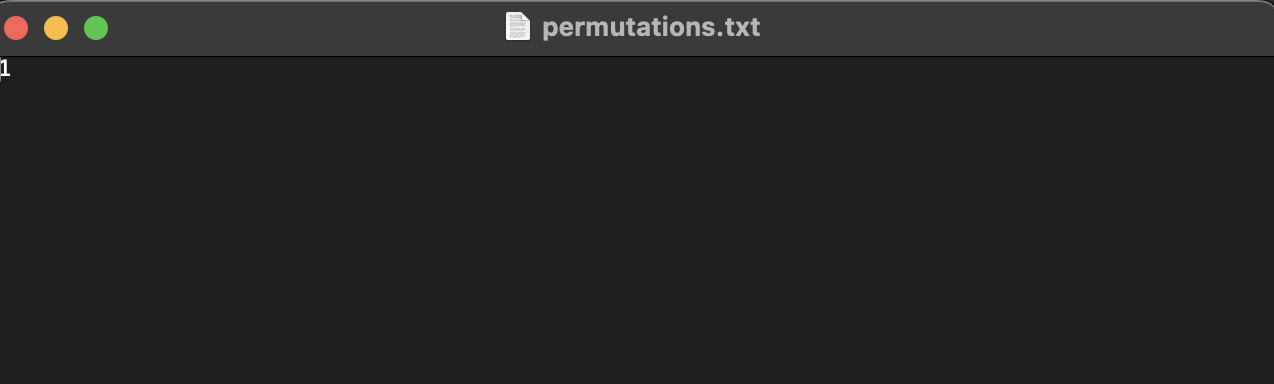
\includegraphics[scale=0.6]{First.png}}
  		\caption{Пример работы 1}
	\end{figure}
	\newpage
	\item $N=2$, то есть дерево из 2 вершин.
	\begin{figure}[h]
  		\center{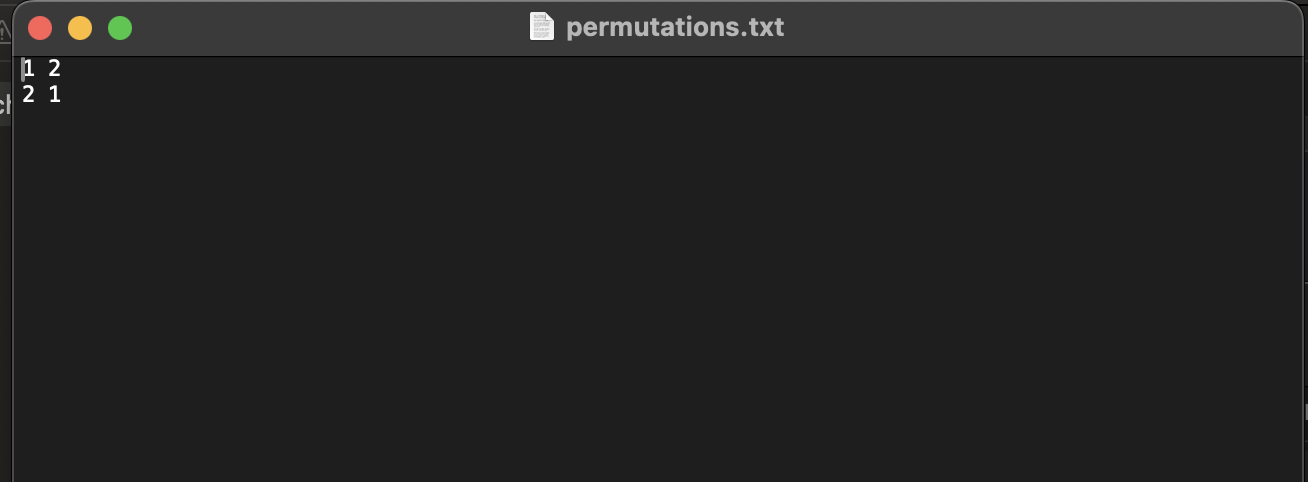
\includegraphics[scale=0.6]{Second.png}}
  		\caption{Пример работы 2}
	\end{figure}
	\item $N=3$, то есть дерево из 3 вершины.
	\begin{figure}[h]
  		\center{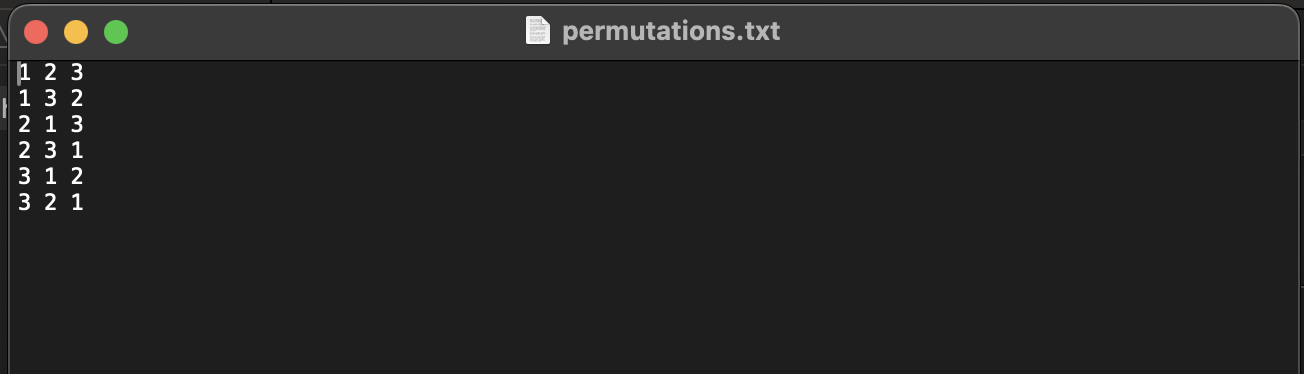
\includegraphics[scale=0.6]{Third.png}}
  		\caption{Пример работы 3}
	\end{figure}
	\newpage
	\item $N=4$, то есть дерево из 4 вершины.
	\begin{figure}[h]
  		\center{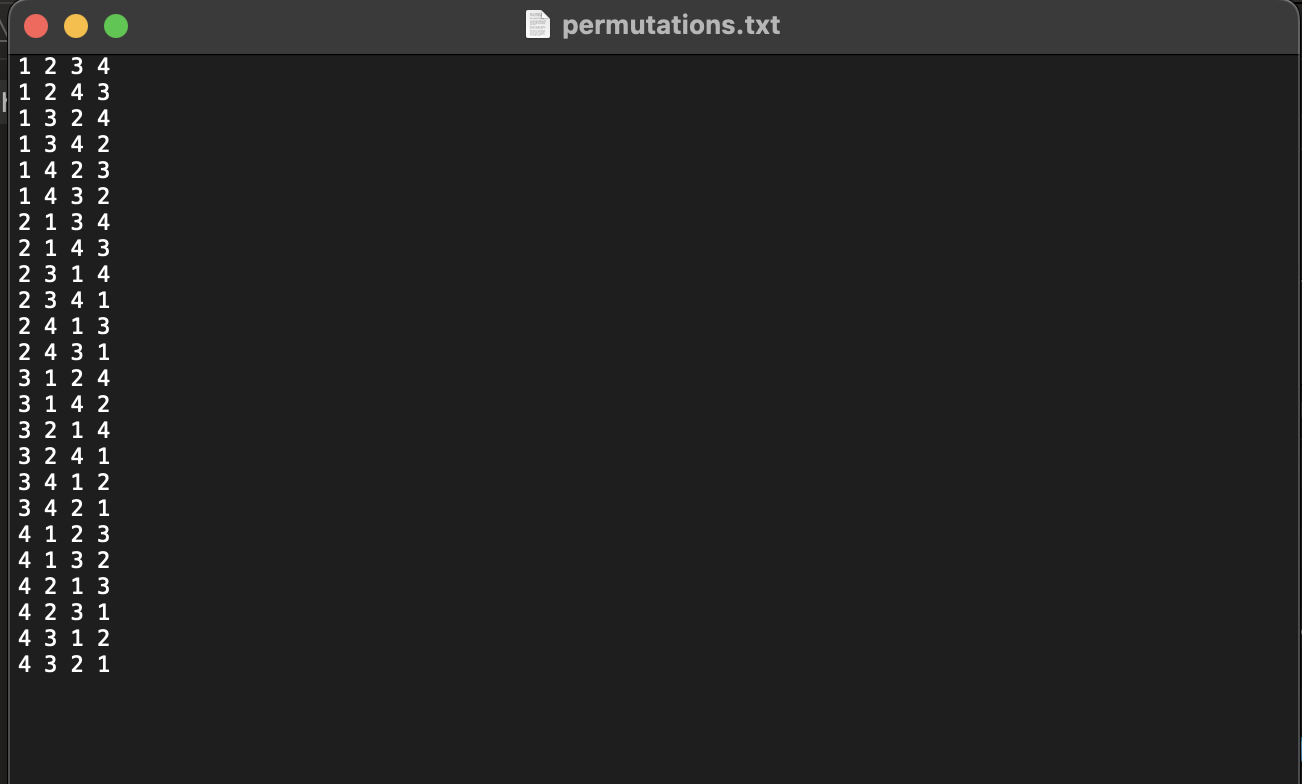
\includegraphics[scale=0.6]{Fourth.png}}
  		\caption{Пример работы 4}
	\end{figure}
\end{enumerate}
\newpage
\section*{Заключение}
\addcontentsline{toc}{section}{Заключение}
Цель достигнута: изучен и реализован метод полного перебора, 
проведен анализ эффективности. Метод полного перебора предполагает 
перебор всех возможных комбинаций вершин, что является 
вычислительно затратной операцией. Однако он гарантирует 
нахождение оптимального решения в контексте задачи обхода вершин 
графа.
\end{document}